
\stopthumb
\chapter{Anhang}
\includegraphics[scale=0.4]{"Bilder Kapitel/Anhang"}

\newpage
\section{Bingo}
Versuche, in so viele Kästchen wie möglich eine Unterschrift zu bekommen. Aber: Eine Person darf auf 
Deinem Blatt höchstens zwei Mal ihren Namen schreiben. Wenn Du eine Längs-, Quer- oder Diagonallinie 
fertig hast, rufe laut:1 \textbf{Bingo!} \\
\begin{center}
    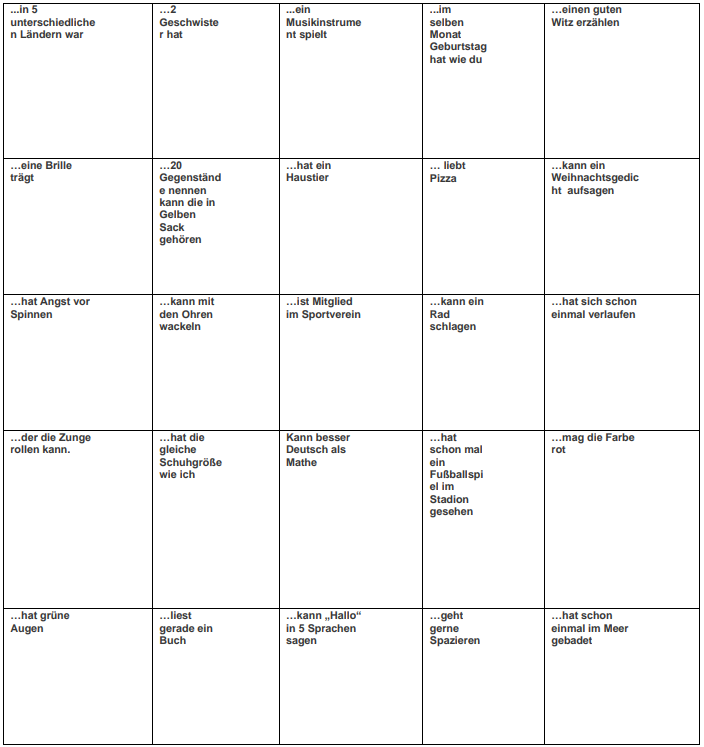
\includegraphics[scale=0.9]{Anhang/Bingo.png}
\end{center}

\newpage
\section{Stratego}

\includegraphics[scale=0.9]{Anhang/Stratego.png}
\newpage

\section{Familie Meyer}

\begin{center}
    

\resizebox{\textwidth - 1cm}{!}{
\begin{tabular}{|c|c|c|c|c|}
   \hline
    & & & & \\ 
    & & & & \\ 
        Familie Maier & Familie Maier & Familie Maier & Familie Maier & Familie Maier \\
        & & & & \\ 
         & & & & \\ \hline
        & & & & \\ 
        & & & & \\ 
        Familie Mayer & Familie Mayer & Familie Mayer & Familie Mayer & Familie Mayer \\
        & & & & \\ 
         & & & & \\ \hline
        & & & & \\ 
        & & & & \\ 
        Familie Meier & Familie Meier & Familie Meier & Familie Meier & Familie Meier \\
        & & & & \\ 
         & & & & \\ \hline
                 & & & & \\ 
        & & & & \\ 
        Familie Meyer & Familie Meyer & Familie Meyer & Familie Meyer & Familie Meyer \\
        & & & & \\ 
         & & & & \\ \hline
                 & & & & \\ 
        & & & & \\ 
        Familie Mair & Familie Mair & Familie Mair & Familie Mair & Familie Mair \\
        & & & & \\ 
         & & & & \\ \hline
                 & & & & \\ 
        & & & & \\ 
        Familie Meir & Familie Meir & Familie Meir & Familie Meir & Familie Meir \\
        & & & & \\ 
         & & & & \\ \hline
                 & & & & \\ 
        & & & & \\ 
        Familie Mayr & Familie Mayr & Familie Mayr & Familie Mayr & Familie Mayr \\
        & & & & \\ 
         & & & & \\ \hline
                          & & & & \\ 
        & & & & \\ 
        Familie Meyr & Familie Meyr & Familie Meyr & Familie Meyr & Familie Meyr \\
        & & & & \\ 
         & & & & \\ \hline
\end{tabular}}
\end{center}
\newpage
\section{Besuch im Zoo}
%\resizebox{\textwidth - 1cm}{!}{
\begin{table}[h]
    \centering
    \begin{tabular}{|c|c|c|c|c|}
    \hline
        
\includegraphics[width=2.5cm]{Anhang/Reh.png}&
\includegraphics[width=2.5cm]{Anhang/Reh.png} & 
\includegraphics[width=2.5cm]{Anhang/Reh.png}&
\includegraphics[width=2.5cm]{Anhang/Reh.png} & 
\includegraphics[width=2.5cm]{Anhang/Reh.png} \\ \hline
                
\includegraphics[width=2.5cm]{Anhang/Löwe.png}&
\includegraphics[width=2.5cm]{Anhang/Löwe.png} & 
\includegraphics[width=2.5cm]{Anhang/Löwe.png}&
\includegraphics[width=2.5cm]{Anhang/Löwe.png} & 
\includegraphics[width=2.5cm]{Anhang/Löwe.png} \\ \hline
                
\includegraphics[width=2.5cm]{Anhang/Elefant.png}&
\includegraphics[width=2.5cm]{Anhang/Elefant.png} & 
\includegraphics[width=2.5cm]{Anhang/Elefant.png}&
\includegraphics[width=2.5cm]{Anhang/Elefant.png} & 
\includegraphics[width=2.5cm]{Anhang/Elefant.png} \\ \hline
                        
\includegraphics[width=2.5cm]{Anhang/Schildkröte.png}&
\includegraphics[width=2.5cm]{Anhang/Schildkröte.png} & 
\includegraphics[width=2.5cm]{Anhang/Schildkröte.png}&
\includegraphics[width=2.5cm]{Anhang/Schildkröte.png} & 
\includegraphics[width=2.5cm]{Anhang/Schildkröte.png} \\ \hline
            
\includegraphics[width=2.5cm]{Anhang/Schlange.png}&
\includegraphics[width=2.5cm]{Anhang/Schlange.png} & 
\includegraphics[width=2.5cm]{Anhang/Schlange.png}&
\includegraphics[width=2.5cm]{Anhang/Schlange.png} & 
\includegraphics[width=2.5cm]{Anhang/Schlange.png} \\ \hline
        
\includegraphics[width=2.5cm]{Anhang/Hase.png}&
\includegraphics[width=2.5cm]{Anhang/Hase.png} & 
\includegraphics[width=2.5cm]{Anhang/Hase.png}&
\includegraphics[width=2.5cm]{Anhang/Hase.png} & 
\includegraphics[width=2.5cm]{Anhang/Hase.png} \\ \hline
        
\includegraphics[width=2.5cm]{Anhang/Fisch.png}&
\includegraphics[width=2.5cm]{Anhang/Fisch.png} & 
\includegraphics[width=2.5cm]{Anhang/Fisch.png}&
\includegraphics[width=2.5cm]{Anhang/Fisch.png} & 
\includegraphics[width=2.5cm]{Anhang/Fisch.png} \\ \hline
    \end{tabular}

\end{table}
\newpage
\begin{table}[h]
	\centering
	\begin{tabular}{|c|c|c|c|c|}
		\hline
		
\includegraphics[width=2.5cm]{Anhang/Marienkäfer.jpg}&
\includegraphics[width=2.5cm]{Anhang/Marienkäfer.jpg} & 
\includegraphics[width=2.5cm]{Anhang/Marienkäfer.jpg}&
\includegraphics[width=2.5cm]{Anhang/Marienkäfer.jpg} & 
\includegraphics[width=2.5cm]{Anhang/Marienkäfer.jpg} \\ \hline
		
\includegraphics[width=2.5cm]{Anhang/Kräbs.jpg}&
\includegraphics[width=2.5cm]{Anhang/Kräbs.jpg} & 
\includegraphics[width=2.5cm]{Anhang/Kräbs.jpg}&
\includegraphics[width=2.5cm]{Anhang/Kräbs.jpg} & 
\includegraphics[width=2.5cm]{Anhang/Kräbs.jpg} \\ \hline
		
\includegraphics[width=2.5cm]{Anhang/Igel.jpg}&
\includegraphics[width=2.5cm]{Anhang/Igel.jpg} & 
\includegraphics[width=2.5cm]{Anhang/Igel.jpg}&
\includegraphics[width=2.5cm]{Anhang/Igel.jpg} & 
\includegraphics[width=2.5cm]{Anhang/Igel.jpg} \\ \hline
		
\includegraphics[width=2.5cm]{Anhang/Oktopus.jpg}&
\includegraphics[width=2.5cm]{Anhang/Oktopus.jpg} & 
\includegraphics[width=2.5cm]{Anhang/Oktopus.jpg}&
\includegraphics[width=2.5cm]{Anhang/Oktopus.jpg} & 
\includegraphics[width=2.5cm]{Anhang/Oktopus.jpg} \\ \hline
		
\includegraphics[width=2.5cm]{Anhang/Vogel.jpg}&
\includegraphics[width=2.5cm]{Anhang/Vogel.jpg} & 
\includegraphics[width=2.5cm]{Anhang/Vogel.jpg}&
\includegraphics[width=2.5cm]{Anhang/Vogel.jpg} & 
\includegraphics[width=2.5cm]{Anhang/Vogel.jpg} \\ \hline
		
\includegraphics[width=2.5cm]{Anhang/Wurm.jpg}&
\includegraphics[width=2.5cm]{Anhang/Wurm.jpg} & 
\includegraphics[width=2.5cm]{Anhang/Wurm.jpg}&
\includegraphics[width=2.5cm]{Anhang/Wurm.jpg} & 
\includegraphics[width=2.5cm]{Anhang/Wurm.jpg} \\ \hline
	\end{tabular}
	
\end{table}
%}
\newpage

\section{Pärchen Suchspiel}
\begin{center}
    

\resizebox{\textwidth - 1cm}{!}{
\begin{tabular}{|c|c|c|c|c|}
   \hline

    & & & & \\ 
        Romeo & Julia & Bibi & Tina & Tom \\

         & & & & \\ \hline

        & & & & \\ 
        Jerry & Tim & Struppi & Barbie & Ken \\
         & & & & \\ \hline
        & & & & \\ 
        Adam & Eva & Asterix & Obelix & Max \\
         & & & & \\ \hline
        & & & & \\ 
        Moritz & Timon & Pumba & Batman & Robin \\
         & & & & \\ \hline
        & & & & \\ 
        Bonni & Clyde & Hänsel & Gretel & Dick \\
         & & & & \\ \hline
        & & & & \\ 
        Doof & Cap & Capper & Cesare & Cleopatra \\
         & & & & \\ \hline
        & & & & \\ 
        Ernie & Bert & Homer & Marge & Sissi \\
         & & & & \\ \hline
        & & & & \\ 
        Franz & Tarzan & Jane & Mickey & Mini \\
         & & & & \\ \hline
\end{tabular}}
\end{center}

\newpage
\section{Vorstellen mit Zettel ziehen}
\begin{table}[h]
    \Large
    \begin{tabular}{|l|}
    \hline
     Was ist das lauteste Geräusch, welches Du jemals gehört hast?  \\ \hline
     Was ist Deine früheste Erinnerung in Deinem Leben? \\ \hline
     Was würdest Du Dir für diese Gruppe hier wünschen?  \\ \hline
     Nenne alle Orte in welchen Du schon gelebt hast!  \\ \hline
     Was ist die lustigste Filmszene, die Du je gesehen hast? \\ \hline
     Wie war Dein Spitzname als Kind? \\ \hline
     Was war Dein schlimmstes Erlebnis bei einem Unwetter?  \\ \hline
     Was war Dein schönstes Erlebnis auf einer anderen Freizeit?  \\ \hline
     Wo ist Dein Lieblingsplatz in der Natur?  \\ \hline
     Was ist Deine Lieblingsmahlzeit?  \\ \hline
     Was ist Deine Lieblingsmusik? \\ \hline
     Was war das bisher ungewöhnlichste Erlebnis in Deinem Leben?  \\ \hline
     Was war das bisher schrecklichste Erlebnis in Deinem Leben?  \\ \hline
     Was war das bisher schönste Erlebnis in Deinem Leben? \\ \hline
     Was war die beste Note in der Schule und in welchem Fach?  \\ \hline
     Welcher Popstar würdest du am liebsten auch sein?  \\ \hline
     Welcher Fußballer würdest du am liebsten auch sein? \\  \hline
     Wenn Du jemand anderes sein könntest, wer würdest Du am liebsten sein? \\ \hline
    \end{tabular}
\end{table}
\newpage
\section{Mafia}
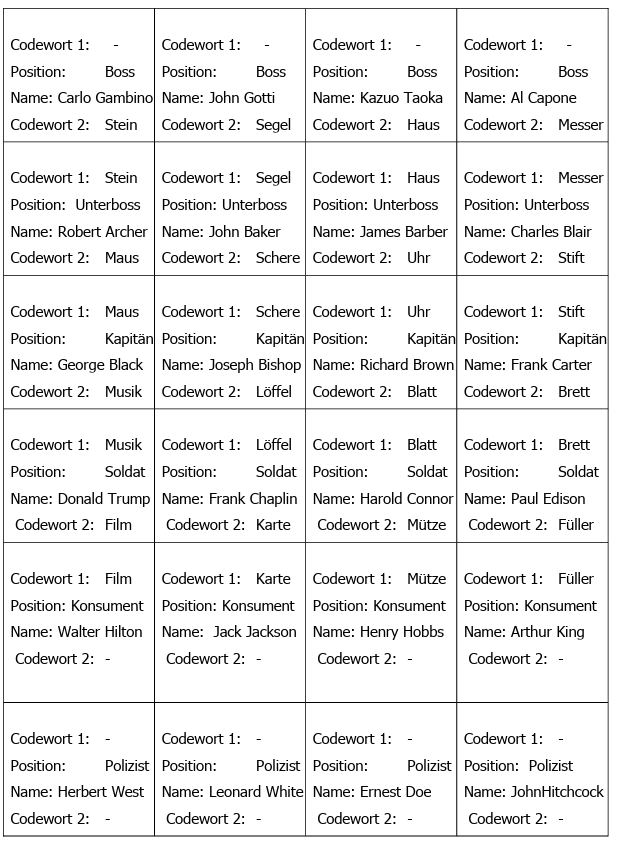
\includegraphics[scale=1]{Anhang/Mafia.png}



